\noindent surgical low-level tasks done with rest position trick (joining, patch, complex cutting/suturing)
\begin{itemize}
  \item describe the particular tasks and show that the essence is the same,
  \item describe our method with all the tricks
  \item include a schematic illustration
\end{itemize}
\begin{figure}[!h]
\begin{center}
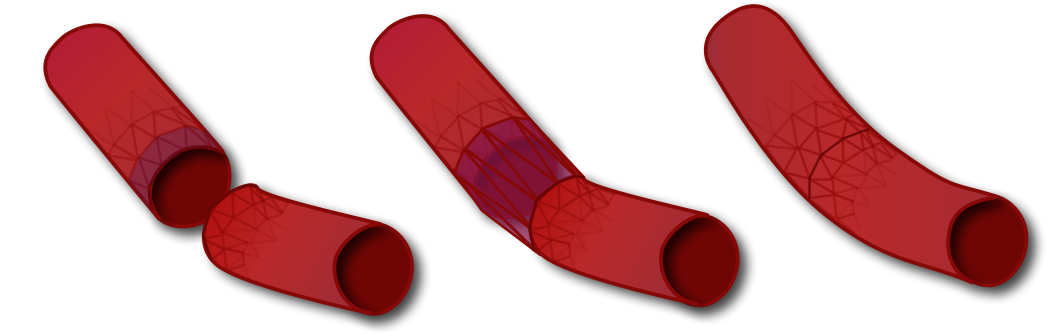
\includegraphics[width=\columnwidth]{img/rest_shape_scheme.png}
\end{center}
\caption{Scheme showing the method for joining two vessels.}
\label{JoiningVessels}
\end{figure}